\subsection{Руководство пользователя}
\subsubsection{Установка программного обеспечения}
Для работы программного обеспечения требуется ПЭВМ с установленной ОС Windows 7 и выше и наличием .NET Framework 4.5. Программное обеспечение представлено в виде нескольких файлов динамических библиотек (DLL) и файла приложения (\textit{Thesis.App.exe}). Для установки программы на компьютер достаточно скопировать данные файлы в любую папку на ПЗУ. Имя и расположение папки не имеет значения. На этом установку системы можно считать законченной.

\subsubsection{Формат входных данных}
Для работы программы требуется минимум два файла: файл с описанием параметров векторов и файл с обучающей выборкой для номинального режима работы системы.

Во всех файлах существует возможность оставлять однострочные комментарии. Комментарий начинается с символа „\%“ и продолжается до конца строки. При чтении файлов программой комментарии игнорируются.

Файл с описанием параметров должен заполняться следующим образом. Каждый параметр представляется файле отдельной строкой, которая имеет формат:

\textsf{[весовой коэффициент] : имя : описание\_параметра}

Разделителями в данном файле служат двоеточие, точка с запятой и запятая. Весовой коэффициент является необязательным параметром.

Если параметр не должен учитываться программой, указывается ключевое слово \textit{ignorefeature}.

Пример: \textsf{time : ignorefeature}

Поддерживаются следующие типы параметров:
\begin{itemize}
	\item непрерывные (ключевое слово \textit{continuous}). \\ Пример: \textsf{pressure : continuous}
	\item дискретные с фиксированным множеством значений. Для таких параметров все возможные значения указываются после имени. \\ Пример: \textsf{state : opened, closed}
	\item дискретные с открытым множеством значений (ключевое слово \textit{discrete}). Для таких параметров системы сама определяет возможные значения на основе данных из обучающих выборок. \\ Пример: \textsf{orbit : discrete}
\end{itemize}

Файлы с данными обучающих выборок представляют собой набор строк (записей), каждая из которых представляет собой вектор с набором значений. Значения в строке разделяются запятыми или точками с запятой. Количество, состав и тип значений должны строго соответствовать указанным в файле с описанием параметров.

Пример записи:

\textsf{16:39:50, 45.5, opened, high}

\subsubsection{Запуск программного обеспечения}
Исполняемым файлом программы является файл \textit{Thesis.App.exe}. Программа при запуске принимает на вход параметры, указанные в таблице~\ref{tab:spec:AppOptions}.

Пример команды запуска:

\texttt{thesis.app fields.txt -r nominal1.txt nominal2.txt [-a regime1.txt regimeN.txt] [-f threshold 0.5] [-d kmeans] [-m sqreuclid] [-n standard]}

Если программа запущена без параметров либо параметры указаны неверно, то будет выведена справочная информация о параметрах, как показано на рисунке~\ref{fig:spec:scr:AppHelp}.

\begin{figure}[h]
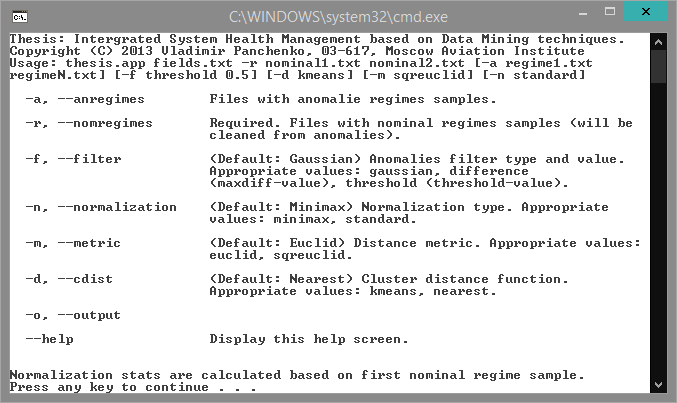
\includegraphics[width=0.7\textwidth]{scr_app_help}
\caption{Экран со справочной информацией}
\label{fig:spec:scr:AppHelp}
\end{figure}

\begin{table}[h]
\caption{Параметры запуска программы}
\label{tab:spec:AppOptions}

\begin{tabular}{|C{125pt}|C{255pt}|C{95pt}|}
\hline
Формат & Описание & Обязательный \\
\hline
имя\_файла & Файл с описанием формата параметров векторов. & Да \\
\hline
-r имя\_файла1 \dots имя\_файлаN & Файлы с обучающими выборками для номинальных режимов работы системы & Да \\
\hline
-a имя\_файла1 \dots имя\_файлаN & Файлы с обучающими выборками для внештатных (аномальных) режимов работы системы & Нет \\
\hline
-f тип\_фильтра [параметр\_фильтра] & Тип фильтра, использующегося при удалении аномалий из обучающих выборок. Допустимые значения: gaussian (гауссовый), difference (разностный), threshold (пороговый). Для разностного фильтра необходимо указать максимальную разность, для пороговго - величину порога. Значение по умолчанию: gaussian. & Нет \\
\hline
-n вид\_нормализации & Вид нормализации (масштабирования) векторов с данными. Допустимые значения: minimax (минимаксная), standard (по стандартному отклонению). Значение по умолчанию: minimax. & Нет \\
\hline
-m тип\_метрики & Тип метрики пространства. Допустимые значения: euclid (евклидова), sqreuclid (квадрат евклидовой). Значение по умолчанию: euclid. & Нет \\
\hline
-d тип\_расстояния & Тип функции для измерения расстояния между кластером и вектором. Допустимые значения: kmeans (до центра кластера), nearest (до ближайшей точки кластера). Значение по умолчанию: nearest. & Нет \\
\hline
-o имя\_файла & Имя файла для сохранения вывода программы. & Нет \\
\hline
\end{tabular}
\end{table}

\subsubsection{Работа с программным обеспечением}
Если все параметры для запуска были указаны корректно, программа запрашивает у пользователя ввод порогового значения $\varepsilon$, как показано на рисунке~\ref{fig:spec:scr:EnterEpsilon}.

\begin{figure}[h]
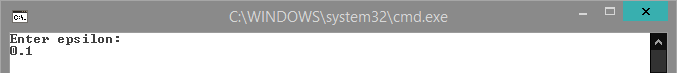
\includegraphics[width=0.7\textwidth]{scr_app_epsilon}
\caption{Экран со справочной информацией}
\label{fig:spec:scr:EnterEpsilon}
\end{figure}